% !TeX program = lualatex
% GenerationClosureGC.tex
% 生成と閉包の双対性 — ガロア対応による統一的理論
%
% 著者: Claude (TeXファイル生成) & Antigravity (Leanファイル生成)
% 日付: 2025-12-26

\documentclass[a4paper,11pt]{ltjsarticle}

% ===== パッケージ =====
\usepackage{amsmath,amssymb,amsthm}
\usepackage{mathtools}
\usepackage{tikz}
\usetikzlibrary{arrows.meta,positioning,matrix,decorations.pathmorphing,calc,shapes.geometric}
\usepackage{tikz-cd}
\usepackage{hyperref}
\usepackage{cleveref}
\usepackage{tcolorbox}
\tcbuselibrary{theorems,skins,breakable}

% ===== 定理環境 =====
\theoremstyle{definition}
\newtheorem{definition}{定義}[section]
\newtheorem{theorem}[definition]{定理}
\newtheorem{lemma}[definition]{補題}
\newtheorem{proposition}[definition]{命題}
\newtheorem{corollary}[definition]{系}
\newtheorem{example}[definition]{例}
\newtheorem{remark}[definition]{注意}

% ===== tcolorbox による強調ボックス =====
\newtcolorbox{keybox}[1][]{
  colback=blue!5!white,
  colframe=blue!75!black,
  fonttitle=\bfseries,
  title={#1},
  breakable
}

\newtcolorbox{leanbox}[1][]{
  colback=gray!5!white,
  colframe=gray!75!black,
  fonttitle=\ttfamily\bfseries,
  title={Lean 4 形式化: #1},
  breakable
}

% ===== マクロ =====
\newcommand{\N}{\mathbb{N}}
\newcommand{\layer}{\mathrm{layer}}
\newcommand{\rank}{\mathrm{rank}}
\newcommand{\closure}{\mathrm{closure}}
\newcommand{\minLayer}{\mathrm{minLayer}}
\newcommand{\sSup}{\mathrm{sSup}}
\newcommand{\Set}{\mathrm{Set}}
\newcommand{\Finset}{\mathrm{Finset}}
\newcommand{\WithTop}{\mathrm{WithTop}}

% ===== タイトル =====
\title{%
  \textbf{生成と閉包の双対性}\\[0.5em]
  \large ガロア対応による統一的理論とLean 4形式化
}
\author{%
  Claude \textit{(TeXファイル生成)}\\
  Antigravity \textit{(Leanファイル生成)}
}
\date{2025年12月26日}

\begin{document}

\maketitle

\begin{abstract}
本稿では、構造塔（Structure Tower）における\textbf{生成}（ランク）と\textbf{閉包}の間のガロア対応を数学的に解説する。
この対応は、線形代数における次元・生成系、位相空間論における閉包、集合論における累積階層など、
多くの数学的構造に共通する「階層的構成」の本質を捉えている。
理論はLean 4で形式化されており、ニコラ・ブルバキの『数学原論』における「母構造」の精神に従う。
\end{abstract}

\tableofcontents

% =====================================
\section{序論}
% =====================================

\subsection{動機と背景}

数学において、集合を「段階的に構成する」という考え方は普遍的に現れる：

\begin{itemize}
  \item \textbf{線形代数}: ベクトル空間の生成系から次元が定まり、部分空間の閉包（生成する部分空間）が得られる
  \item \textbf{位相空間論}: 集合の閉包は、その集合を含む最小の閉集合である
  \item \textbf{集合論}: フォン・ノイマン宇宙 $V_\alpha$ における集合のランクと、累積階層
  \item \textbf{確率論}: フィルトレーション（情報系）における可測性の時刻とマルチンゲールの停止時刻
\end{itemize}

これらに共通する構造を抽出し、\textbf{ガロア対応}として統一的に理解することが本稿の目標である。

\subsection{本稿の構成}

\begin{enumerate}
  \item \S\ref{sec:structure-tower}: 構造塔とその基本性質
  \item \S\ref{sec:galois}: ランク・閉包のガロア対応
  \item \S\ref{sec:lanes}: 3つの実装レーン（Finset, Set, WithTop）
  \item \S\ref{sec:closure-operator}: 閉包演算子の性質
  \item \S\ref{sec:lean}: Lean 4形式化の概要
\end{enumerate}

% =====================================
\section{構造塔}\label{sec:structure-tower}
% =====================================

\subsection{定義}

\begin{definition}[構造塔]
\textbf{最小層付き構造塔}（Structure Tower with Minimum Layer）は、以下のデータからなる：
\begin{enumerate}
  \item 台集合 $X$（carrier）
  \item 順序集合 $I$（Index、時刻・段階を表す）
  \item 層関数 $\layer : I \to \mathcal{P}(X)$
  \item 最小層関数 $\minLayer : X \to I$
\end{enumerate}

これらは以下の公理を満たす：
\begin{enumerate}
  \item \textbf{被覆性}: $\forall x \in X, \exists i \in I, x \in \layer(i)$
  \item \textbf{単調性}: $i \le j \Rightarrow \layer(i) \subseteq \layer(j)$
  \item \textbf{最小性（所属）}: $\forall x \in X, x \in \layer(\minLayer(x))$
  \item \textbf{最小性（極小）}: $x \in \layer(i) \Rightarrow \minLayer(x) \le i$
\end{enumerate}
\end{definition}

\begin{figure}[htbp]
\centering
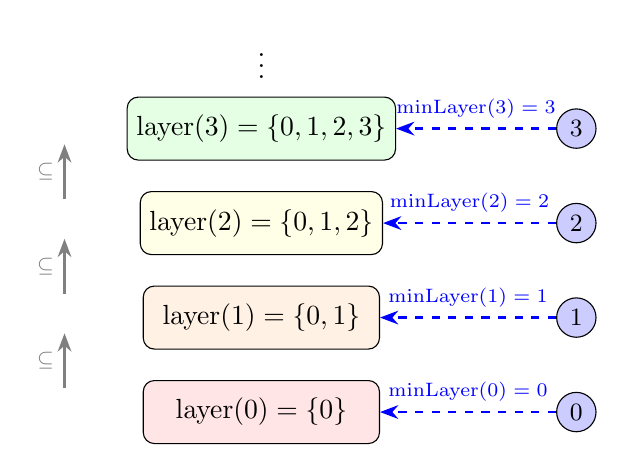
\begin{tikzpicture}[
  layer/.style={draw, rounded corners, minimum width=3cm, minimum height=0.8cm, align=center},
  element/.style={circle, draw, fill=blue!20, minimum size=0.5cm, inner sep=1pt, font=\small},
  arrow/.style={-{Stealth}, thick}
]
  % Layers
  \node[layer, fill=red!10] (L0) at (0, 0) {$\layer(0) = \{0\}$};
  \node[layer, fill=orange!10] (L1) at (0, 1.2) {$\layer(1) = \{0, 1\}$};
  \node[layer, fill=yellow!10] (L2) at (0, 2.4) {$\layer(2) = \{0, 1, 2\}$};
  \node[layer, fill=green!10] (L3) at (0, 3.6) {$\layer(3) = \{0, 1, 2, 3\}$};
  \node at (0, 4.5) {$\vdots$};
  
  % Elements with minLayer
  \node[element] (e0) at (4, 0) {$0$};
  \node[element] (e1) at (4, 1.2) {$1$};
  \node[element] (e2) at (4, 2.4) {$2$};
  \node[element] (e3) at (4, 3.6) {$3$};
  
  % Arrows showing minLayer
  \draw[arrow, dashed, blue] (e0) -- (L0) node[midway, above, font=\scriptsize] {$\minLayer(0) = 0$};
  \draw[arrow, dashed, blue] (e1) -- (L1) node[midway, above, font=\scriptsize] {$\minLayer(1) = 1$};
  \draw[arrow, dashed, blue] (e2) -- (L2) node[midway, above, font=\scriptsize] {$\minLayer(2) = 2$};
  \draw[arrow, dashed, blue] (e3) -- (L3) node[midway, above, font=\scriptsize] {$\minLayer(3) = 3$};
  
  % Monotonicity arrows
  \draw[arrow, gray] (-2.5, 0.3) -- (-2.5, 1) node[midway, left, font=\scriptsize] {$\subseteq$};
  \draw[arrow, gray] (-2.5, 1.5) -- (-2.5, 2.2) node[midway, left, font=\scriptsize] {$\subseteq$};
  \draw[arrow, gray] (-2.5, 2.7) -- (-2.5, 3.4) node[midway, left, font=\scriptsize] {$\subseteq$};
\end{tikzpicture}
\caption{自然数塔 $\mathrm{natTowerMin}$ の構造。$\layer(n) = \{k \mid k \le n\}$, $\minLayer = \mathrm{id}$}
\label{fig:nat-tower}
\end{figure}

\subsection{正規形補題}

以下の補題は、理論全体の基礎となる：

\begin{keybox}[正規形補題（Normal Form Lemma）]
\begin{lemma}\label{lem:normal-form}
任意の構造塔において、
\[
  x \in \layer(i) \iff \minLayer(x) \le i
\]
\end{lemma}
\end{keybox}

\begin{proof}
($\Rightarrow$) $x \in \layer(i)$ ならば、最小性（極小）より $\minLayer(x) \le i$。

($\Leftarrow$) $\minLayer(x) \le i$ とする。最小性（所属）より $x \in \layer(\minLayer(x))$。
単調性より $\layer(\minLayer(x)) \subseteq \layer(i)$。よって $x \in \layer(i)$。
\end{proof}

% =====================================
\section{ガロア対応}\label{sec:galois}
% =====================================

\subsection{ランク関数と閉包関数}

\begin{definition}[ランク関数]
集合 $A \subseteq X$ に対して、\textbf{ランク}を次で定義する：
\[
  \rank(A) := \sup \{ \minLayer(x) \mid x \in A \}
\]
これは「$A$ を生成するのに必要な最小の段階」を表す。
\end{definition}

\begin{definition}[閉包関数]
集合 $A \subseteq X$ に対して、\textbf{閉包}を次で定義する：
\[
  \closure(A) := \layer(\rank(A))
\]
\end{definition}

\subsection{ガロア対応の定理}

\begin{keybox}[ガロア対応（Galois Connection）]
\begin{theorem}\label{thm:galois}
ランク関数と層関数は\textbf{ガロア対応}をなす：
\[
  \rank(A) \le i \iff A \subseteq \layer(i)
\]
\end{theorem}
\end{keybox}

\begin{proof}
($\Rightarrow$) $\rank(A) \le i$ とする。任意の $x \in A$ に対して、
\[
  \minLayer(x) \le \sup\{\minLayer(y) \mid y \in A\} = \rank(A) \le i
\]
正規形補題より $x \in \layer(i)$。よって $A \subseteq \layer(i)$。

($\Leftarrow$) $A \subseteq \layer(i)$ とする。任意の $x \in A$ に対して、
$x \in \layer(i)$ より正規形補題で $\minLayer(x) \le i$。
よって $\rank(A) = \sup\{\minLayer(x) \mid x \in A\} \le i$。
\end{proof}

\subsection{図式による理解}

\begin{figure}[htbp]
\centering
\begin{tikzcd}[column sep=large, row sep=large]
  \mathcal{P}(X) \arrow[r, shift left=1.5, "\rank"] \arrow[r, phantom, "\dashv"] 
    & I^{\mathrm{op}} \arrow[l, shift left=1.5, "\layer"]
\end{tikzcd}
\caption{ガロア対応 $\rank \dashv \layer$}
\label{fig:galois}
\end{figure}

\begin{figure}[htbp]
\centering
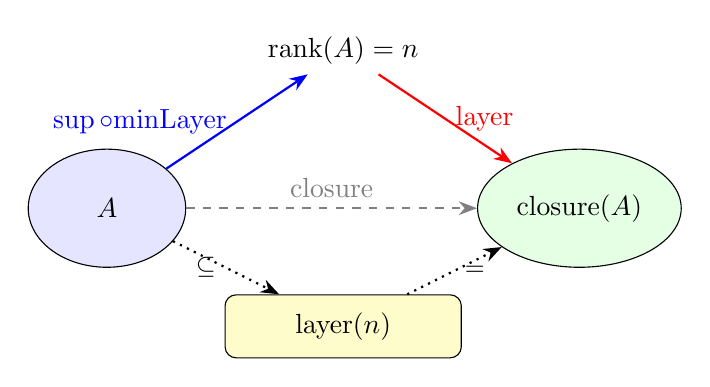
\begin{tikzpicture}[
  set/.style={draw, ellipse, minimum width=2cm, minimum height=1.5cm, align=center},
  layer/.style={draw, rectangle, rounded corners, minimum width=3cm, minimum height=0.8cm, fill=yellow!20},
  arrow/.style={-{Stealth}, thick}
]
  % Sets
  \node[set, fill=blue!10] (A) at (-3, 0) {$A$};
  \node[set, fill=green!10] (clA) at (3, 0) {$\closure(A)$};
  
  % Rank
  \node (rank) at (0, 2) {$\rank(A) = n$};
  
  % Layer
  \node[layer] (layer) at (0, -1.5) {$\layer(n)$};
  
  % Arrows
  \draw[arrow, blue] (A) -- (rank) node[midway, left] {$\sup \circ \minLayer$};
  \draw[arrow, red] (rank) -- (clA) node[midway, right] {$\layer$};
  \draw[arrow, dashed, gray] (A) -- (clA) node[midway, above] {$\closure$};
  
  % Subset relations
  \draw[arrow, dotted] (A) -- (layer) node[midway, left, font=\small] {$\subseteq$};
  \draw[arrow, dotted] (layer) -- (clA) node[midway, right, font=\small] {$=$};
\end{tikzpicture}
\caption{閉包の構成: $\closure(A) = \layer(\rank(A))$}
\label{fig:closure-construction}
\end{figure}

% =====================================
\section{3つの実装レーン}\label{sec:lanes}
% =====================================

形式化においては、インデックス集合 $I$ の取り扱いによって3つの「レーン」を用意している：

\begin{table}[htbp]
\centering
\begin{tabular}{|c|c|c|c|c|}
\hline
\textbf{レーン} & \textbf{Index型} & \textbf{ランク関数} & \textbf{条件} & \textbf{用途} \\
\hline
Lane B (Finset) & $\N$ & \texttt{rankFinNat} & なし & 計算可能 \\
\hline
Lane SetLevel & $\N$ & \texttt{rankSetNat} & Nonempty, BddAbove & 一般集合（有界） \\
\hline
Lane C (WithTop) & $\WithTop(\N)$ & \texttt{rankTop} & \textbf{なし} & 条件なしGC \\
\hline
\end{tabular}
\caption{3つの実装レーン}
\label{tab:lanes}
\end{table}

\subsection{Lane C: 条件なしガロア対応}

Lane C では、$\WithTop(\N) = \N \cup \{\top\}$ を用いることで、
\textbf{空集合や非有界集合にも対応}できる：

\begin{itemize}
  \item $\rank(\emptyset) = \bot = 0$
  \item $\rank(\N) = \top$（非有界）
  \item $\layer(\top) = X$（全体集合）
\end{itemize}

\begin{theorem}[条件なしガロア対応]
Lane C において、任意の集合 $A \subseteq \N$ と $i \in \WithTop(\N)$ に対して、
\[
  \rank(A) \le i \iff A \subseteq \layer(i)
\]
が\textbf{無条件で}成り立つ。
\end{theorem}

\subsection{レーン間の整合性}

\begin{proposition}[レーン整合補題]
有限集合 $s \in \Finset(\N)$ に対して、
\[
  \mathrm{rankTop}(\uparrow s) = \uparrow(\mathrm{rankFinNat}(s))
\]
ここで $\uparrow$ はそれぞれ $\Set$ への埋め込みと $\WithTop$ への埋め込みを表す。
\end{proposition}

% =====================================
\section{閉包演算子の性質}\label{sec:closure-operator}
% =====================================

ガロア対応から、閉包が\textbf{閉包演算子}の公理を満たすことが自動的に導かれる。

\begin{theorem}[閉包演算子の性質]
$\closure : \mathcal{P}(X) \to \mathcal{P}(X)$ は以下を満たす：
\begin{enumerate}
  \item \textbf{拡大性（Extensivity）}: $A \subseteq \closure(A)$
  \item \textbf{単調性（Monotonicity）}: $A \subseteq B \Rightarrow \closure(A) \subseteq \closure(B)$
  \item \textbf{冪等性（Idempotence）}: $\closure(\closure(A)) = \closure(A)$
\end{enumerate}
\end{theorem}

\begin{proof}
すべての性質はガロア対応\textbf{のみ}から導かれる。

\textbf{拡大性}: $\rank(A) \le \rank(A)$ より、GC の右向きで $A \subseteq \layer(\rank(A)) = \closure(A)$。

\textbf{単調性}: $A \subseteq B$ とする。GC より
$\rank(A) \le \rank(B)$。$\layer$ の単調性より $\closure(A) \subseteq \closure(B)$。

\textbf{冪等性}: 
\begin{itemize}
  \item ($\supseteq$) 拡大性より $\closure(A) \subseteq \closure(\closure(A))$。
  \item ($\subseteq$) GC の左向きより $\layer(i) \subseteq \layer(i)$ から
    $\rank(\layer(i)) \le i$。よって
    $\rank(\closure(A)) = \rank(\layer(\rank(A))) \le \rank(A)$。
    $\layer$ の単調性より $\closure(\closure(A)) \subseteq \closure(A)$。
\end{itemize}
\end{proof}

\begin{remark}[GC-only 証明の重要性]
上記の証明は $\rank(\layer(i)) = i$ という等式（自然数塔では成り立つ）を使わず、
\textbf{不等式 $\rank(\layer(i)) \le i$ のみ}で完結している。
これにより、より一般の構造塔への拡張が可能となる。
\end{remark}

% =====================================
\section{Lean 4 形式化}\label{sec:lean}
% =====================================

以下に、主要な定義と定理のLean 4コードを示す。

\begin{leanbox}[正規形補題]
\begin{verbatim}
theorem mem_layer_iff_minLayer_le {x : T.carrier} {i : T.Index} :
    x ∈ T.layer i ↔ T.minLayer x ≤ i := by
  constructor
  · intro hx
    exact T.minLayer_minimal x i hx
  · intro hle
    have hmem : x ∈ T.layer (T.minLayer x) := T.minLayer_mem x
    exact T.monotone hle hmem
\end{verbatim}
\end{leanbox}

\begin{leanbox}[ガロア対応（Lane C）]
\begin{verbatim}
theorem rankTop_le_iff {A : Set ℕ} {i : WithTop ℕ} :
    rankTop A ≤ i ↔ A ⊆ layerTop i := by
  constructor
  · intro hrank x hx
    match i with
    | ⊤ => exact Set.mem_univ x
    | (n : ℕ) =>
      have hmem : minLayerTop x ∈ minLayerTop '' A := ⟨x, hx, rfl⟩
      have hle : minLayerTop x ≤ (n : WithTop ℕ) := calc
        minLayerTop x ≤ sSup (minLayerTop '' A) := le_sSup hmem
        _ = rankTop A := rfl
        _ ≤ n := hrank
      simp only [minLayerTop, coe_le_coe] at hle
      exact mem_layerNat_iff.mpr hle
  · intro hsub
    apply sSup_le
    rintro j ⟨x, hx, rfl⟩
    have hxmem : x ∈ layerTop i := hsub hx
    match i with
    | ⊤ => exact le_top
    | (n : ℕ) =>
      simp only [layerTop] at hxmem
      exact coe_le_coe.mpr (mem_layerNat_iff.mp hxmem)
\end{verbatim}
\end{leanbox}

\begin{leanbox}[閉包演算子インスタンス]
\begin{verbatim}
noncomputable def closureTopOp : ClosureOperator (Set ℕ) where
  toFun := closureTop
  monotone' := fun _ _ h => closureTop_mono h
  le_closure' := subset_closureTop
  idempotent' := closureTop_idem
\end{verbatim}
\end{leanbox}

% =====================================
\section{結論と展望}
% =====================================

\subsection{達成したこと}

\begin{enumerate}
  \item 構造塔における\textbf{ランク・閉包のガロア対応}を厳密に定式化
  \item \textbf{3つの実装レーン}（Finset, Set, WithTop）の提供
  \item Lane C における\textbf{条件なしガロア対応}の実現
  \item \textbf{閉包演算子}の性質をGC-onlyで証明（一般化可能）
  \item Lean 4による\textbf{完全な形式化}（sorry なし）
\end{enumerate}

\subsection{今後の発展}

\begin{itemize}
  \item 一般の \texttt{StructureTowerWithMin} への理論の輸出
  \item 確率論における停止時刻との対応の形式化
  \item 圏論的な観点からの再構成（閉包演算子をコモナドとして）
\end{itemize}

% =====================================
\appendix
\section{記号一覧}

\begin{tabular}{ll}
$\layer(i)$ & 層 $i$ に属する要素の集合 \\
$\minLayer(x)$ & 要素 $x$ が初めて現れる最小の層 \\
$\rank(A)$ & 集合 $A$ のランク（$\sup \{\minLayer(x) \mid x \in A\}$）\\
$\closure(A)$ & 集合 $A$ の閉包（$\layer(\rank(A))$）\\
$\WithTop(\N)$ & $\N \cup \{\top\}$、完備束をなす \\
$\dashv$ & ガロア対応（左随伴 $\dashv$ 右随伴）\\
\end{tabular}

\end{document}
